\documentclass[12pt, letterpaper]{article}
\usepackage[utf8]{inputenc}
\usepackage{natbib}
\usepackage{graphicx}

\graphicspath{{./figures/}}

\title{Literature Review}

\author{Shreyas Kalvankar \and Hrushikesh Pandit \and Pranav Parwate \and Atharva Patil}

\begin{document}
	\maketitle
	
	\begin{abstract}
		Astronomical imaging has made stupendous progress through the years with more and more sophisticated techniques being introduced with every new telescope launch. The rise in computation power enabled astronomers to increase the number of observations and resulted in flooding of information that could be processed as quickly as it could be seen by the human eye. The data albeit abundant, is computationally expensive to process and remains dormant in the archives globally. One such example being the Hubble Legacy Archive where there are hundreds and thousands of snapshots taken by the Hubble Space telescope which lie unprocessed in the database but can be of astronomical significance. This document summarizes a brief study of generative adversarial networks and convolutional neural networks and different techniques belonging to the disciplines that can be applied to astronomical images to make them usable for astronomical inspection. 
	\end{abstract}
	
	\section{Introduction}
		\hspace*{0.25 in}Hubble Legacy Archive or HLA is a project which endeavours to complement the Hubble Space Telescope by augmenting the HST Data Archive and providing superior browsing and searching capabilities. A large amount of raw images remain unprocessed in the HLA, never seen by a human eye. These raw images are typically low resolution, black and white and unfit to work with in today's day and age. It takes hundreds of hours to process them.
	\section{Hubble Legacy Archive}
		\hspace*{0.25 in}In the past decade, astronomical research was extensively performed using large catalogs which were search-able. This was made possible due to advances in computer technology and databases. The biggest challenge that is faced today is to convert this  large unstructured database into a comprehensive catalog. Advances in relational databases technology has made it efficient to create and store and search large catalogs. 

Sloan Digital Sky Survey or SDSS, was one such catalog. It uniformly observed the regions of the sky in a certain filter band at regular intervals of time. The HST however, has targeted only particular sources.

The Hubble Space Telescope (often referred to as HST or Hubble) is a space telescope that was launched into low Earth orbit in 1990 and remains in operation. It was not the first space telescope, but it is one of the largest and most versatile, well known both as a vital research tool and as a public relations boon for astronomy.

The Hubble Space Telescope archive was an archive for the Hubble Space Telescope which was launched in low Earth orbit back in 1990. It is an important tool for research and is the one of the biggest and most versatile telescopes which is active today.
The Hubble Legacy Archive (HLA) endeavors to create calibrated scientific data from the Hubble Space Telescope archive and make them accessible via user-friendly and Virtual Observatory (VO) compatible interfaces. 

	\section{Image Colorization}
	\subsection{Hint Based Colorization}
		\hspace*{0.25 in} Automated colorization of gray scale images has been researched extensively throughout the machine learning community and is more specifically studied by those who indulge in the discipline of computer vision. Apart from being visually fascinating, it has many other applications ranging from restoration to enhancement for better interpretability.\\
		\hspace*{0.25 in}\cite{levin2004colorization} proposed using colorization hints from the user in a quadratic cost function which imposed that neighboring pixels in space-time with similar intensities should have similar colours. This was a simple but effective method but only had hints which were provided in form of imprecise colored scribbles on the grayscale input image. But with no additional information about the image, the method was able to efficiently generate high quality colorizations. \cite{huang2005edge} addressed the color bleeding issue faced in this approach and solved it using adaptive edge detection. \cite{yatziv2006chrominance} used luminescence based weighting for hints to boost efficiency. \cite{qu2006manga} extended the original cost function to enforce color continuity over similar textures along with intensities.\\
		\hspace*{0.25 in}\cite{welsh2002color} had proposed another approach that reduced the burden on the user by only requiring a full color example of an image with similar composition. It matched the texture and luminescence between the example and the target grayscale image and received realistic results as long as the example image was sufficiently similar.\\
		\hspace*{0.25 in}Regardless of the scribble based or example based approach, the algorithms still needed sufficient human assistance in form of hand drawn or colorized images. 
		\begin{figure}
		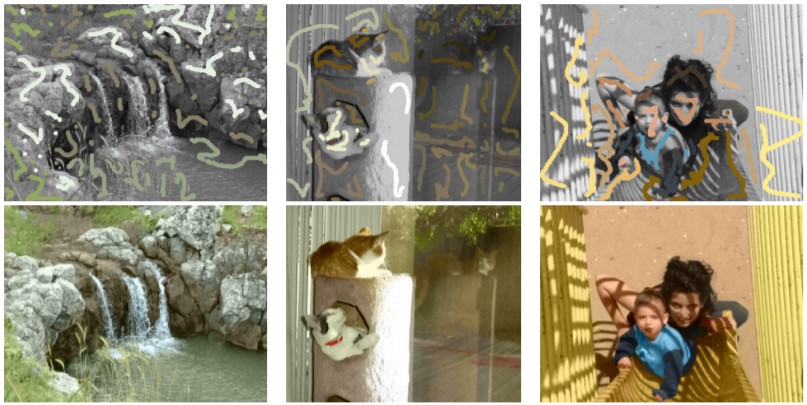
\includegraphics[width=\textwidth]{levin_scribble_based_colorization_example.jpg}
		\caption{Example of Scribble based colorization \citep{levin2004colorization}}
		\label{fig: levin_example}
		\end{figure}
		\subsection{Deep Colorization}
		\hspace*{0.25 in}Owing to recent advances, the Convolutional Neural Networks are a de facto standard for solving image classification problems and their popularity continues to rise with continual improvements. CNNs are peculiar in their ability to learn and differentiate colors, patterns and shapes within an image and their ability to associate them with different classes.\\
		\hspace*{0.25 in}\cite{cheng2016deep} proposed a per pixel training for neural networks using DAISY \citep{tola2008descriptor}, and semantic \citep{long2015semantic} features to predict the chrominance value for each pixel, that used bilateral filtering to smooth out accidental image artifacts. With a large enough dataset, this method proved to be superior to the example based techniques even with a simple Euclidean loss function against the ground truth values.\\
		\hspace*{0.25 in}Finally, \cite{dahl2016automatic} successfully implemented a system to automatically colorize black \& white images using several ImageNet-trained layers from VGG-16 \cite{simonyan2015deep} and integrating them with auto-encoders that contained residual connections. These residual connections merged the outputs produced by the encoding VGG16 layers and the decoding portion of the network in the later stages. \cite{he2015deep} showed that deeper neural networks can be trained by reformulating layers to learn residual function with reference to layer inputs. Using this \textit{Residual Connections}, \cite{he2015deep} created the \textit{ResNets} that went as deep as 152 layers and won the 2015 ImageNet Challenge.
		\subsection{Generative Adversarial Networks}
		\hspace*{0.25 in}\cite{goodfellow2014generative} introduced the adversarial framework that provides an approach to training a neural network which uses the generative distribution of $p_g(x)$ over the input data $x$.\\
		\hspace*{0.25 in}Since it's inception in 2015, many extended works of GAN have been proposed over years including DCGAN \citep{radford2016unsupervised}, Conditional-GAN \citep{mirza2014conditional}, iGAN \citep{zhu2018generative}, Pix2Pix \citep{isola2018imagetoimage}.\\
		\hspace*{0.25 in}\cite{radford2016unsupervised} applied the adversarial framework for training convolutional neural networks as generative models for images, demonstrating the viability of \textit{deep convolutional generative adversarial networks}.\\
		\hspace*{0.25 in}DCGAN is the standard architecture to generate images from random noise. Instead of generating images from random noise, Conditional-GAN \citep{mirza2014conditional} uses a condition to generate output image. For e.g. a grayscale image is the condition for colorization of image. Pix2Pix \citep{isola2018imagetoimage} is a Conditional-GAN with images as the conditions. Besides learning the mapping from input image to output image, it can also learn a separate loss function to train this mapping. Pix2Pix is considered to be the state of the art architecture for image-image translation problems like colorization.
		
\renewcommand\bibname{References}
\bibliographystyle{apalike}
\bibliography{References}

\end{document}